\section{Stoßprozess bei zwei Pendeln}
	
	Dieser Versuch dient zur Betrachtung der Stoßgesetze. Dazu wird ein ballistischer zentraler Stoß mit Hilfe von zwei aufgehängten Massen untersucht. Es stellt sich die Frage, wie genau die Stoßgesetze für das Verhältnis der Massen mit den gemessenen Werten übereinstimmen. Das Ergebnis dieser Messung zeigt die Übereinstimmung von Theorie und den ermittelten Werten. 
	
	\subsection{Methoden}
		
		\subsubsection{Aufbau}
			
		Zum Messen wird der im Folgenden dargestellte Aufbau verwendet. Hierbei handelt es sich um zwei Pendel an denen Kugeln mit unterschiedlicher Masse angehängt sind. Hierbei besitzt die kleinere Kugel die Masse $m_1$ und die Größere folglich $m_2$. Die Schwerpunkte dieser Kugeln liegen auf einer Geraden, sodass ein ballistischer zentraler Stoß durch das Auslenken eines Pendels möglich ist. 
		Für die Pendel werden die Fäden so aufgehängt, dass deren Enden jeweils auf gleicher Höhe befestigt sind. Die Massen werden dann mittig, jeweils auf einen Faden, gehängt, sodass die Auslenkungen in einer Ebene stattfinden können. In Abbildung \ref{abb:VersuchsskizzeStoss} ist der Aufbau skizziert. In Ruhelage berühren sich die Kugeln an dem Punkt $a_0$. Des weiteren sind die Positionen $a_1$ und $a_2$ die Punkte von denen aus die Auslenkungen bestimmt werden. Diese unterscheiden sich um den Durchmesser der jeweiligen Kugel von $a_0$.
		\begin{figure}[ht]
			\centering
			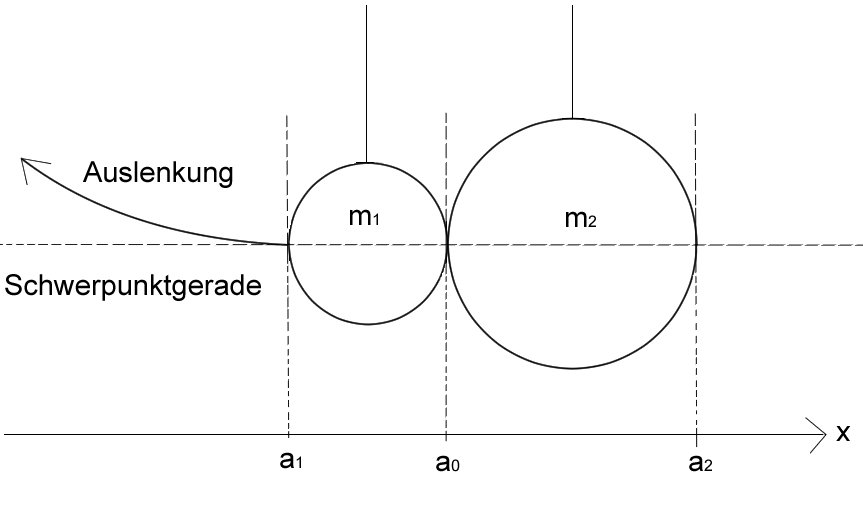
\includegraphics[width=\textwidth]{Kugelstoss.png}
			\caption{Skizzierung des Versuchsaufbaus}
			\label{abb:VersuchsskizzeStoss}	
		\end{figure}
		Dies wird so gewählt, damit das Messen leichter fällt. Für die Messung der Auslenkungen werden Schiebeblöcke verwendet (vgl. Abb. \ref{abb:VersuchsaufbauStoss}), welche sich auf einem Maß frei bewegen lassen. Damit sind $a_1'$ und $a_2'$ nach dem initialen Stoß in guter Näherung zu bestimmen. Die gestrichenen Variablen sollen hierbei die Auslenkungen nach dem Stoß beschreiben. Zur Bestimmung dieser wird die Differenz zwischen den mit den Schiebeblöcken bestimmten Werte und der Position in Ruhelage gebildet. 
		
		Es werden bei dem Versuch die Auslenkungen $a_1'$ und $a_2'$ für fünf verschiedene Startauslenkungen von $a_1$ und $a_2$ jeweils fünf mal gemessen, wobei die fünf Messwerte für dieselben Auslenkungen gemittelt werden.
		Zudem werden die Pendellänge und Masse der Kugeln bei beiden Pendeln gemessen. Ersteres mit Hilfe eines Maßbands und letzteres über eine Waage.	
		Mit Hilfe der Theorie hinter dem ballistischen zentralen Stoß wird das Massenverhältnis durch die gemessenen Werte bestimmt und dann mit dem Verhältnis der gemessenen Massen verglichen.
				
		\subsubsection{Unsicherheiten}
		
			Zur Berechnung der Unsicherheiten für die gemessenen und ermittelten Werte dient folgende Formel: 
			\begin{equation*}
				u(s) = \pm \sqrt{\sum_{k=0}^{N}\left( \frac{\partial f}{\partial x_i}u(x_i)\right) ^2}. \label{eq:kombUnsicherheit}
			\end{equation*}
			Für die von dem Maß(band) abgelesenen Werte werden Unsicherheiten über eine Dreiecksverteilung und für die von der Waage gemessenen Werte eine Rechteckverteilung verwendet. 
	
	\subsection{Messung}
	
		\subsubsection{Aufnahme der Messwerte}
		
			Für die Pendellängen wurden die Abstände zwischen den Schwerpunkten und den Befestigungshöhen gemessen. 
			Um die Radien der kugelförmigen Massen zu bestimmen, wurde der Umfang dieser gemessen. Die Werte der Pendellängen, der Radien, der gewogenen Massen und Startpunkte sind in Tabelle \ref{tab:Messwerte} dargestellt. Die Unsicherheit für die Radien steht in direktem Zusammenhang mit der Unsicherheit der Umfänge, also der des Maßbandes.
			\begin{table}[ht]
				\caption{Messwerte der Pendellänge, Masse und der Radien}
				\centering
				\label{tab:Messwerte}
				\begin{tabular}{c|l|l}
					{} & {Pendel 1} & {Pendel 2}	\\
					\hline
					{Pendellänge} & {$L_1 = \SI{185+-0,02}{\cm}$} & {$L_2 = \SI{189+-0,02}{\cm}$}	\\
					\hline
					{Kugelmasse} & {$m_1 = \SI{191,47+-0,003}{\g}$} & {$m_2 = \SI{510,21+-0,003}{\g}$}	\\	
					\hline
					{Kugelradien} & {$r_1 = \SI{1,83+-0,003}{\cm}$} & {$r_2 = \SI{2,55+-0,003}{\cm}$}	\\
							
				\end{tabular}
			\end{table}
			
			Wie in Abb. \ref{abb:VersuchsskizzeStoss} eingezeichnet, beschreiben $a_0$, $a_1$ und $a_2$  die Positionen zu Beginn der Messung. Im Laborbuch sind nur die Positionen über dem Maß nach der Auslenkung notiert, jedoch nicht die Auslenkungen selber. Zur Bestimmung dieser für beide Massen wird die Differenz zwischen den Startwerten und den gemittelten Messwerten gebildet. Die dadurch ermittelten Werte sind in Tabelle \ref{tab:Messwerte2} zu finden. Dabei ergeben sich die Unsicherheiten durch die der Startwerte, beim differenzieren, sowie der bei dem Mitteln entstandenen kombinierten Unsicherheit, welche sich aus fünf mal der Unsicherheit des Maßes, sowie einer zusätzlichen Unsicherheit für das nach Augenmaß durchgeführte Schieben der Blöcke von \SI{0,05}{\cm} ergibt. Für die Auslenkungen in der Tabelle bezeichnen $a_{1/2}^{*}$ die Startauslenkungen und $a_{1/2}'$ die Auslenkungen nach dem Stoß. Für die Auswertung sind hierbei jedoch nur die Startauslenkung der stoßenden Kugel und die Auslenkung der gestoßenen Kugel relevant. 	
			\begin{table}[ht]
				\caption{Auslenkungen nach Stoß}
				\centering
				\label{tab:Messwerte2}
	
				\begin{tabular}{c|c|c}
					{$a_{1}^{*}$} & {$\bar{a_{1}}'$} & {$\bar{a_{2}}'$}	\\
					\hline
					{\SI{17,14+-0,03}{\cm}} & {\SI{6,66+-0,06}{\cm}} & {\SI{8,82+-0,06}{\cm}}\\
					{\SI{13,14+-0,03}{\cm}} & {\SI{5,6+-0,06}{\cm}} & {\SI{6,40+-0,06}{\cm}}\\
					{\SI{11,14+-0,03}{\cm}} & {\SI{4,76+-0,06}{\cm}} & {\SI{5,62+-0,06}{\cm}}\\
					{\SI{9,14+-0,03}{\cm}} & {\SI{3,78+-0,06}{\cm}} & {\SI{4,40+-0,06}{\cm}}\\
					{\SI{5,14+-0,03}{\cm}} & {\SI{2,3+-0,06}{\cm}} & {\SI{2,32+-0,06}{\cm}}\\		
					\hline 
					& & \\
					{$a_{2}^{*}$} & {$\bar{a_{1}}'$} & {$\bar{a_{2}}'$}	\\
					\hline
					{\SI{10,1+-0,03}{\cm}} & {\SI{14,62+-0,06}{\cm}} & {\SI{4,98+-0,06}{\cm}}\\
					{\SI{8,1+-0,03}{\cm}} & {\SI{11,74+-0,06}{\cm}} & {\SI{4,14+-0,06}{\cm}}\\
					{\SI{6,1+-0,03}{\cm}} & {\SI{9,04+-0,06}{\cm}} & {\SI{3,22+-0,06}{\cm}}\\
					{\SI{4,1+-0,03}{\cm}} & {\SI{6,04+-0,06}{\cm}} & {\SI{2,32+-0,06}{\cm}}\\
					{\SI{2,1+-0,03}{\cm}} & {\SI{3,36+-0,06}{\cm}} & {\SI{1,4+-0,06}{\cm}}\\	
				\end{tabular}	
			\end{table}
	
		\subsubsection{Datenanalyse}	
			
			Ist die kleinere Kugel mit der Masse $m_1$ die Stoßende, so gilt nach den Gesetzen der Impuls- und Energieerhaltung für den Stoß der folgende Zusammenhang zwischen den Auslenkungen der beiden Kugeln:
			\begin{equation}
				a_2' = \frac{2m_\text{1}}{m_\text{1}+m_\text{2}} \cdot a_1^{*}\footnote{Umgekehrt lassen sich die Indizes tauschen, um den Fall für die große Kugel abzudecken.}. \label{eq:ZusammenhangStoss}
			\end{equation}	 
			Aus der Gleichung folgt ein linearer Zusammenhang zwischen $a_2'$ und $a_1^{*}$ mit dem Faktor $\frac{2m_\text{1}}{m_\text{1}+m_\text{2}}$. Dieser wird im Folgenden als $m_\text{i}$ bezeichnet, wohingegen $m_\text{ii}$ durch den Faktor bei dem zweiten Fall, dass die große Kugel stößt, definiert wird. Aus den Messungen lassen sich also durch Auftragen von $a_2'$ gegen $a_1^{*}$ die Größen $m_\text{i}$ bzw. $m_\text{ii}$ für den zweiten Fall bestimmen. Diese sind in den Abbildungen \ref{abb:AuslenkungMittel} und \ref{abb:AuslenkungGross} dargestellt\footnote{Der Fit wurde von dem Programm SciDavis berechnet, dazu wurden die Unsicherheiten der Auslenkung und die Methode der kleinsten Quadrate herangezogen}. Addieren von $m_\text{i}$ und $m_\text{ii}$ liefert:
			\begin{align}
				m_\text{i} + m_\text{ii} \quad = \frac{2m_\text{1}}{m_\text{1}+m_\text{2}} + \frac{2m_\text{2}}{m_\text{2}+m_\text{1}}
										 = \frac{2(m_\text{1}+m_\text{2})}{m_\text{1}+m_\text{2}} 
										 = \quad 2 \label{eq:Add2}
			\end{align}
			Demnach sollte das Addieren der Steigungen ebenfalls 2 ergeben. Für den ersten Fall ergab sich beim Auftragen der Werte eine Steigung von $0,538 \pm 0,007$ und zusammen mit der Steigung aus dem zweiten Fall von $1,411\pm 0,009$ ergibt sich durch Addition ein Wert von $1,949 \pm 0,011 \approx 2$.
			\begin{figure}[ht]
				\centering
				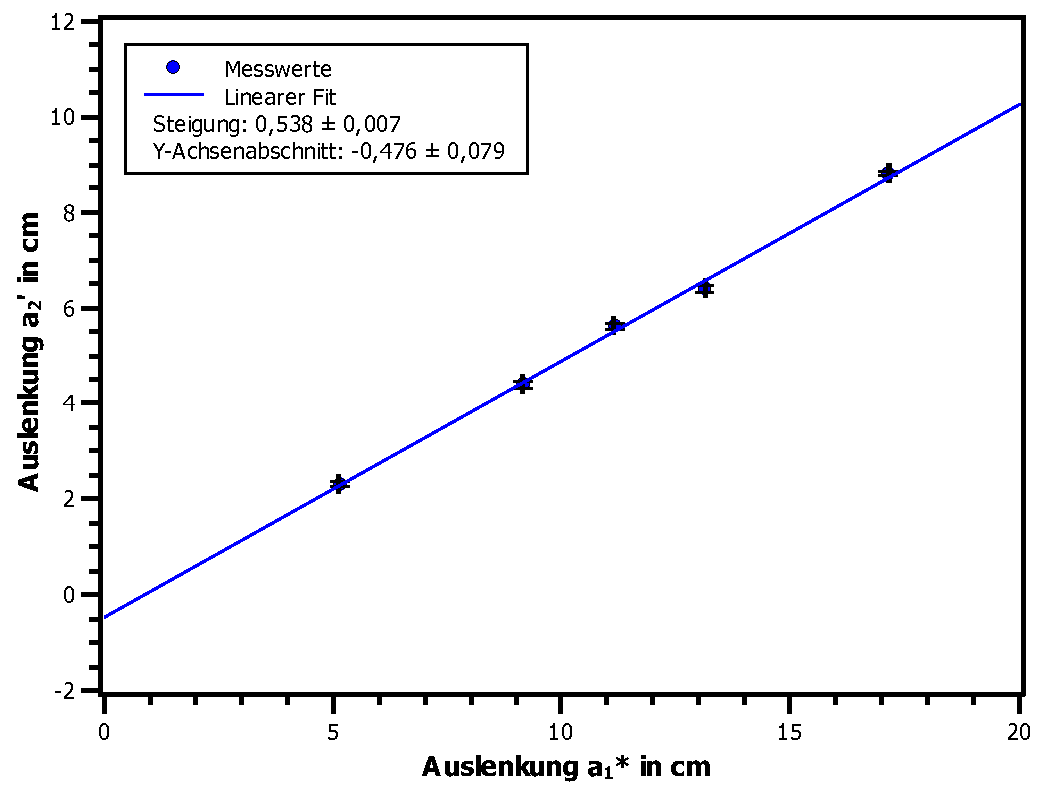
\includegraphics[width=\textwidth]{AuslenkungMittel.pdf}
				\caption{Auslenkungen der größeren Kugel nach Stoß mit der Kleineren}
				\label{abb:AuslenkungMittel}	
			\end{figure}
			\begin{figure}[ht]
				\centering
				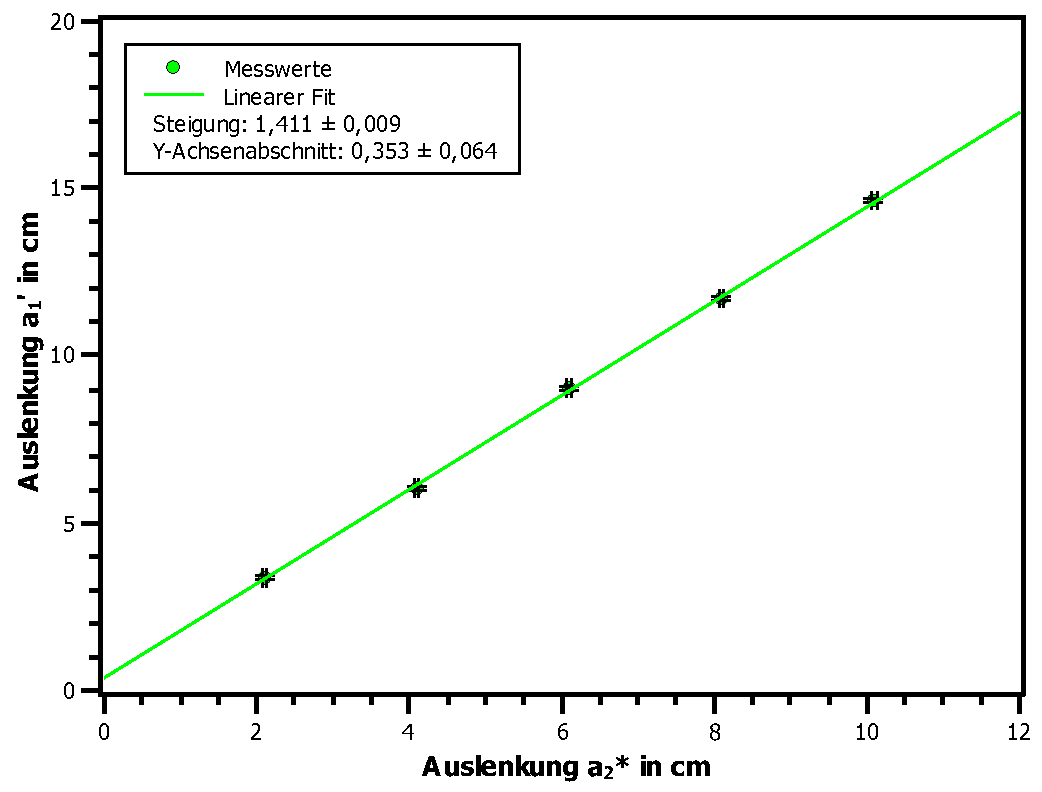
\includegraphics[width=\textwidth]{AuslenkungGross.pdf}
				\caption{Auslenkungen der kleineren Kugel nach Stoß mit der Größeren}
				\label{abb:AuslenkungGross}	
			\end{figure}
		
			Durch Division von $m_\text{i}$ und $m_\text{ii}$ lässt sich das Massenverhältnis durch die Steigungen bestimmen:
			\begin{align}
				\frac{m_\text{i}}{m_\text{ii}} \quad = \frac{2m_\text{1}}{m_\text{1}+m_\text{2}} \cdot \frac{m_\text{2}+m_\text{1}}{2m_\text{2}}
				= \quad  \frac{m_\text{1}}{m_\text{2}} \label{eq:Massenverhältnis}
			\end{align}
			Aus den Steigungen der Graphen folgt durch einsetzen in die Gleichung \ref{eq:Massenverhältnis} ein Massenverhältnis von $0,381 \pm 0,006$ und bei dem dividieren der durch Wiegen gemessenen Massen, welche in Tab. \ref{tab:Messwerte} vorzufinden sind, ein Verhältnis von $0,375$ mit einer vernachlässigbar kleinen Unsicherheit.
			
	\subsection{Diskussion}
		
		Betrachtet man zunächst den linearen Fit für die beiden Messungen, so fällt auf, dass der Y-Achsenabschnitt bei beiden um ungefähr 0,4 von 0 abweicht, was gemäß Gleichung \ref{eq:ZusammenhangStoss} nicht sein sollte. Eine Erklärung dafür wäre, dass bei dieser Messung einige der Startauslenkungen zu groß gewählt wurden und sich der Stoß somit nicht exakt durch die Gleichung \ref{eq:ZusammenhangStoss} beschreiben lässt, da es sich hierbei nicht um einen ballistischen und zentralen Stoß gehandelt haben könnte. Ebenso kann realistisch gesehen kein vollständig elastischer Stoß vorgelegen haben, da Reibung eine Rolle spielt und auch geringfügige Verformung der Metallkugeln zwar vernachlässigbar sind, jedoch auch Einfluss haben könnten.
		Für das durch die Steigungen bestimmte Massenverhältnis ergab sich lediglich eine Abweichung von 1,6\% und bei der Addition nur eine Abweichung von 2,55\% von 2 aus Gleichung \ref{eq:Add2}. Beide Abweichungen sind nahe genug an den zu erwartenden Werten, um die Stoßgesetze mit dieser Messung zu stützen. 
		
	\subsection{Schlussfolgerung}
	
		Im Großen und Ganzen wurde das Ziel dieses Versuches, zu zeigen, dass die Ergebnisse mit der Theorie übereinstimmen, erreicht. Eine Wiederholung des Versuches könnte jedoch zumindest zu besseren Y-Achsenabschnitten für die linearen Fits führen. Hierzu sollten dann weniger starke Auslenkungen gewählt werden und die Messung der Auslenkung, insofern möglich, digitalisiert werden, da das Messen nach Augenmaß mit den Schiebeblöcken als ungenau angenommen werden kann.